\documentclass[tikz,border=10pt]{standalone}
\usepackage{tikz}
\usetikzlibrary{calc}

\begin{document}
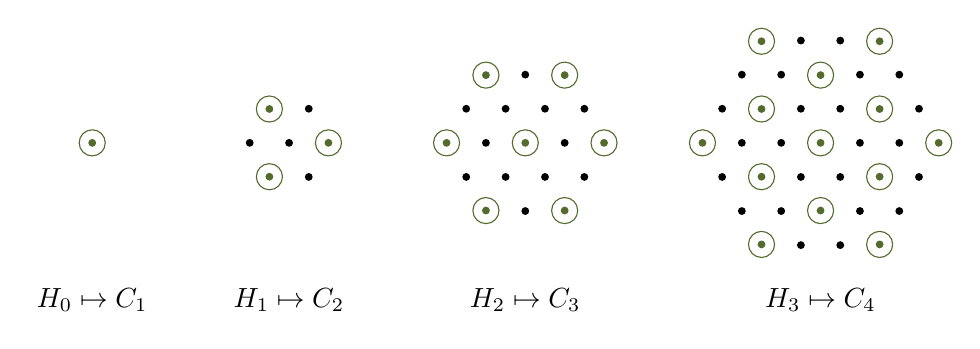
\begin{tikzpicture}[dot/.style={circle, fill=black, inner sep=1pt}]

%─────────────
% Controls
%─────────────
\def\hexstep{0.5}  % Distance from center to first ring point (controls scale)
\definecolor{olivegreen}{rgb}{0.33,0.42,0.18}  % Custom olive green

%─────────────────────────────────────────────────────────────
% Draws a hexagonal lattice of dots:
%─────────────────────────────────────────────────────────────
\newcommand{\drawHexagonDots}[3]{%
  \begin{scope}[shift={({#2},{#3})}]

    \pgfmathtruncatemacro{\rings}{#1}

    \ifnum\rings<1
      \node[dot] at (0,0) {};
    \else
      % Always draw the central dot at the origin
      \node[dot] at (0,0) {};

      % Loop over each ring from 1 to total number
      \foreach \r in {1,...,\rings} {
        \pgfmathsetmacro{\rad}{\r * \hexstep}  % Radius for this ring

        % Each ring has 6 sides (hexagon)
        \foreach \side in {0,...,5} {
          \pgfmathsetmacro{\angleA}{60*\side}
          \pgfmathsetmacro{\angleB}{60*(\side+1)}

          % Define endpoints of one hex side arc at current radius
          \coordinate (A) at (\angleA:\rad);
          \coordinate (B) at (\angleB:\rad);

          % Interpolate points between A and B
          \foreach \k in {0,...,\numexpr\r-1} {
            \pgfmathsetmacro{\t}{\k/\r}
            \path ($(A)!{\t}!(B)$) node[dot] {};
          }
        }
      }
    \fi
  \end{scope}
}

%─────────────
% Draw examples H₁ through H₃
%─────────────
\drawHexagonDots{0}{-4.5}{0}     % H0 = 1
\drawHexagonDots{1}{-2}{0}     % H₁ = 7
\drawHexagonDots{2}{ 1}{0}     % H₂ = 19
\drawHexagonDots{3}{ 4.75}{0}  % H₃ = 37

%─────────────
% Manually draw in selected nodes
%─────────────
\newcommand{\selectPoint}[2]{%
  \node[circle, draw=olivegreen, fill=white] at ({#1},{#2}) {}; 
  \node[dot, fill=olivegreen] at ({#1},{#2}) {}; 
}
%H_0
\selectPoint{-4.5}{0}
%H_1
\selectPoint{-1.5}{0}
\selectPoint{-2.25}{-.43}
\selectPoint{-2.25}{.43}
%H_2
\selectPoint{1}{0}
\selectPoint{2}{0}
\selectPoint{0}{0}
\selectPoint{1.5}{-0.86}
\selectPoint{1.5}{0.86}
\selectPoint{0.5}{-0.86}
\selectPoint{0.5}{0.86}
%H_3
\selectPoint{4.75}{0}
\selectPoint{5.5}{-.43}
\selectPoint{5.5}{.43}
\selectPoint{3.25}{0}
\selectPoint{6.25}{0}
\selectPoint{4}{1.29}
\selectPoint{4}{-1.29}
\selectPoint{5.5}{1.29}
\selectPoint{5.5}{-1.29}
\selectPoint{4}{.43}
\selectPoint{4}{-.43}
\selectPoint{4.75}{.86}
\selectPoint{4.75}{-.86}
% Bad method below 
% \selectPoint{5.25}{0}
% \selectPoint{4.5}{-.43}
% \selectPoint{4.5}{.43}
% \selectPoint{6.25}{0}
% \selectPoint{4}{1.29}
% \selectPoint{4}{-1.29}
% \selectPoint{5}{1.29}
% \selectPoint{5}{-1.29}
% \selectPoint{3.5}{.43}
% \selectPoint{3.5}{-.43}
% \selectPoint{5.75}{.86}
% \selectPoint{5.75}{-.86}

%─────────────
% Labels
%─────────────
\node at (-4.5,-2) {$H_0 \mapsto C_1$};
\node at (-2,-2) {$H_1 \mapsto C_2$};
\node at ( 1,-2) {$H_2 \mapsto C_3$};
\node at ( 4.75,-2) {$H_3 \mapsto C_4$};

\end{tikzpicture}
\end{document}